\documentclass[12pt]{article}
% \textwidth 15.5cm \oddsidemargin 0cm \topmargin -2cm \textheight
% 24cm \footskip 1cm
\usepackage[british]{babel}
\usepackage{epsfig}
\usepackage{amsmath,graphicx,psfrag,pstricks,float,amssymb,fancyhdr,pdfpages, hyperref, enumitem, listings, subcaption, minted, diagbox, appendix, lastpage, biblatex}
% \usepackage[sorting=none]{biblatex}
\usepackage[margin=25mm]{geometry}

% \pagestyle{fancy}
% \pagenumbering{arabic}
% \fancyhead[L]{}
% \cfoot{\thepage}
\pagestyle{fancy}
\fancyhf{}
\fancyfoot[C]{Page \thepage\ of \pageref{LastPage}}
% \setlength{\headheight}{15pt}
\renewcommand{\headrulewidth}{0pt}
\linespread{1.3}  % "One-and-a-half" spacing

\def\n{\noindent}
\def\u{\underline}
\def\hs{\hspace}
\newcommand{\thrfor}{.^{\displaystyle .} .}
%\newcommand{\bvec}[1]{{\bf #1}}

\addbibresource{bibliography.bib}

\begin{document}

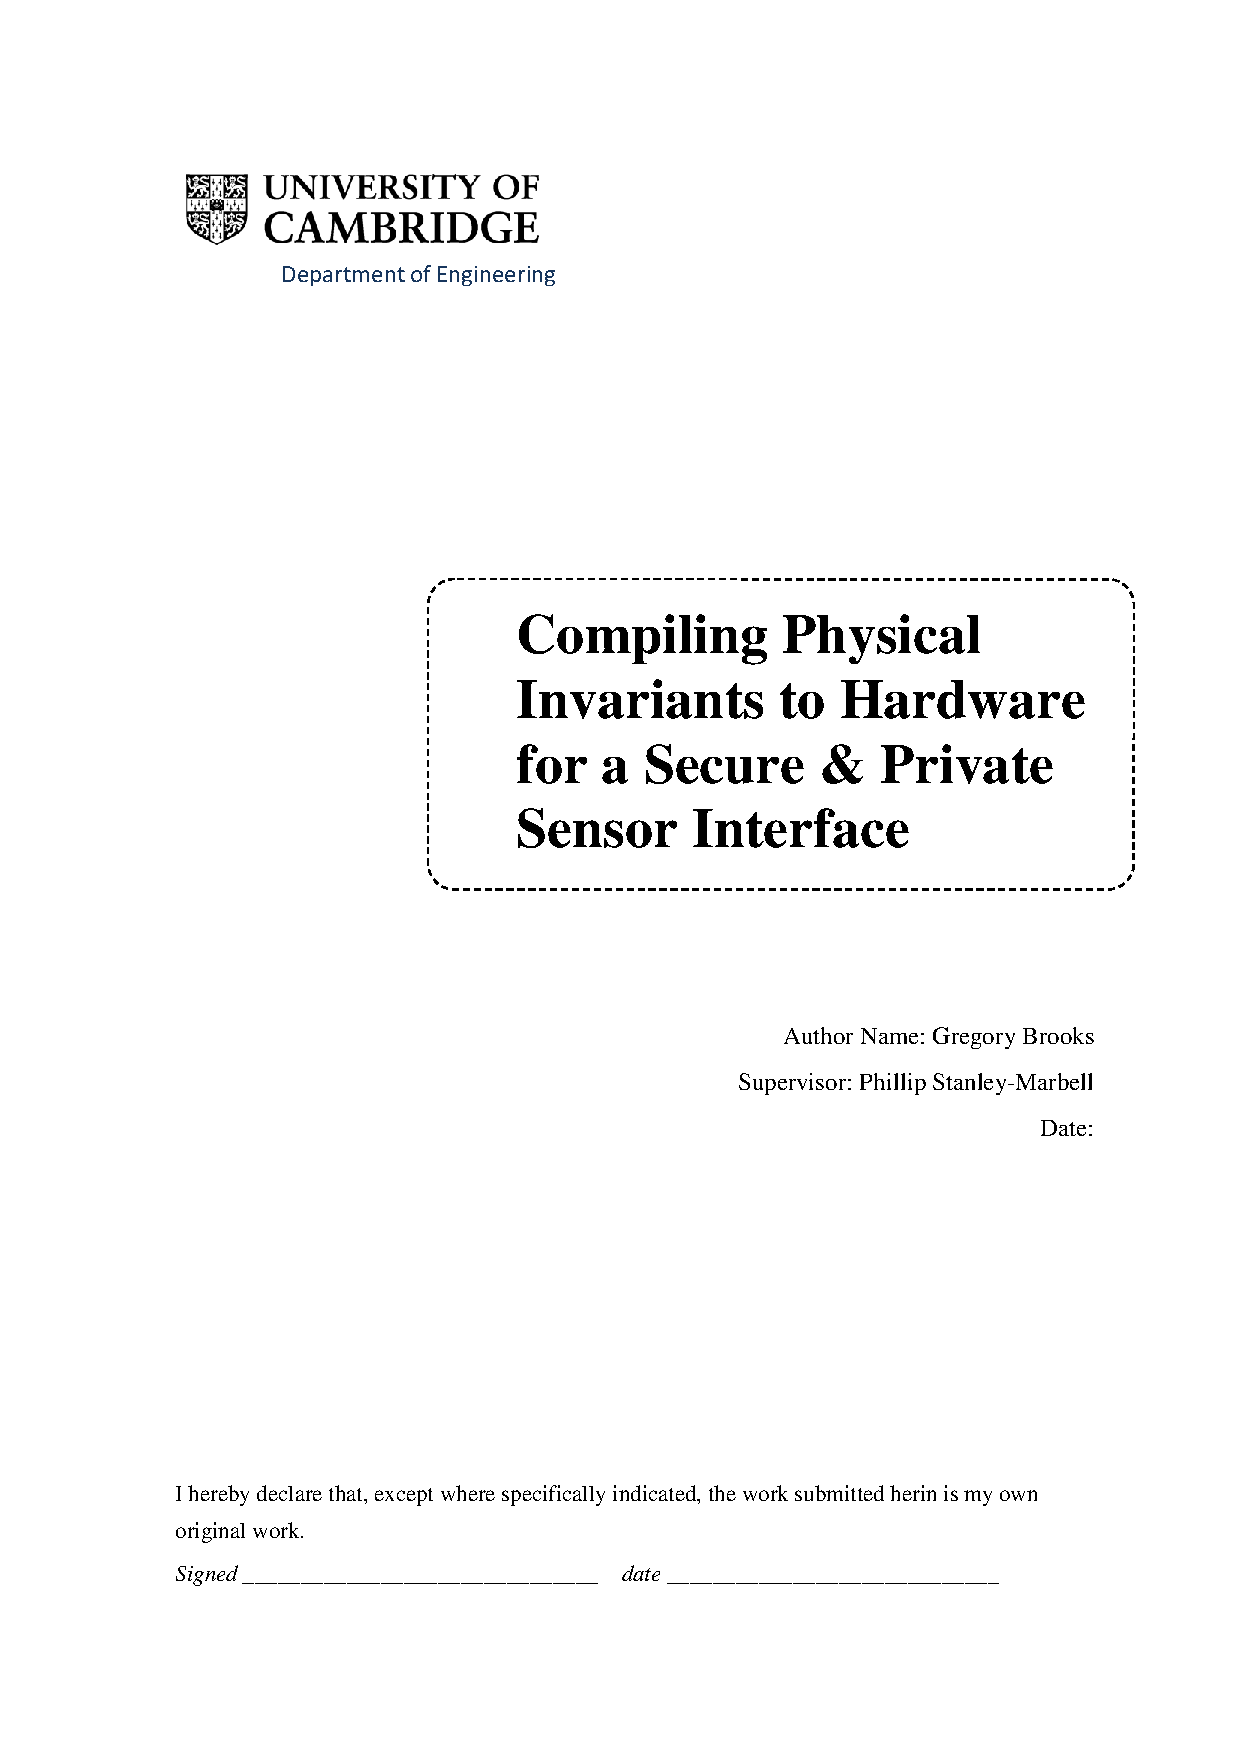
\includepdf[pages={1}]{coversheet.pdf}
\clearpage \mbox{}
\pagenumbering{gobble}
\clearpage
\pagenumbering{arabic}

\noindent

%
% TITLE & CONTENTS PAGE
%

\title
{
  IIB Project Report:\\
  Compiling Physical Invariants to Hardware for a Secure \& Private Sensor Interface\\
}
\author{Gregory Brooks, gb510, Christ's College}
\date{}
\maketitle

\tableofcontents

\pagenumbering{gobble}
\clearpage
\pagenumbering{arabic}

%
% TECHNICAL ABSTRACT
%

\section{Technical Abstract}

\begin{center}
{
  \bf Compiling Physical Invariants to Hardware for a Secure \& Private Sensor Interface\\
}
Gregory Brooks, gb510, Christ's College
\end{center}
\rule{15.7cm}{0.5mm}
\vspace{1cm}


\textit{$\langle$ TODO: write this last$\rangle$}

\newpage



% \clearpage
%
% INTRODUCTION
%

\section{Introduction}

\newpage



%
% THEORRTICAL DEVELOPMENT
%

\section{Theoretical Development}

\newpage



%
% APPARATUS, EQUIPMENT AND EXPERIMENTAL TECHNIQUES
%

\section{Apparatus, Equipment and Experimental Techniques}

\newpage



%
% RESULTS, DELIVERABLES AND DISCUSSION
%

\section{Results, Deliverables and Discussion}

\newpage



%
% CONCLUSIONS
%

\section{Conclusions}

\newpage



\noindent

% Hack to remove REFERENCES REFERENCES header
\markboth{}{}
\printbibliography
\markboth{}{}

\newpage

\begin{appendix}

  %
  % RISK ASSESSMENT RETROSPECTIVE
  %

  \section{Risk Assesment Retrospective}
    The risk assessment submitted at the start of the project does not mention any specific hazards besides office (computer) work, since the project is predominately software/firmware based (all project hardware operated at low voltages i.e. 12V or less). No other hazards were encountered during the course of the project, since the random noise generator PCBs were manufactured by the Dyson Centre's Electronics Development Group. In retrospect, although not part of the initial project specification, the risk assessment could have anticipated the possibility of manufacturing PCBs for the project. The hazards associated with this activity include high temperatures (from a soldering iron/oven/hot air gun) as well as chemical hazards associated with solder, fume extraction etc.



  %
  % UPPER BOUND ON DIFF PRIV
  %

  \section{Derivation of an Upper Bound on Multi-Sensor Differential Privacy Loss}



  %
  % URNG BLOCK DIAGRAM
  %

  \section{Uniform Random Number Generator Block Diagram}
    \textit{$\langle$ TODO: insert block diagram$\rangle$}


  %
  % INVERSION METHOD BLOCK DIAGRAM
  %

  \section{Inversion Method Random Number Generator Block Diagram}
    \textit{$\langle$ TODO: insert block diagram$\rangle$}


  %
  % EUROSYS POSTER
  %

  \section{EuroSys 2019 Poster: Safeguarding Sensor Device Drivers Using Physical Constraints}
    \subsection{Description}
      This poster~\cite{eurosys_poster} was submitted to EuroSys 2019, to communicate the idea of using information about a physical system to condition electronic sensor measurements. The example discussed in the poster is the detection and safeguarding against transduction attacks~\cite{Fu_2018}, where an attacker manipulates a sensor's output to gain control over a system. For example, a presentation~\cite{autonomous_vehicles} illustrates how the proximity sensors on a Tesla vehicle can be fooled into providing erroneous (or even no) data using ultrasonic interference produced by a device built using off-the-shelf electronics. An attacker would not need to have access to the Tesla software (or even physical access to the hardware) in order to control the system's behaviour.

      The poster illustrates how the Newton language can be used to describe a physical system, in this case an accelerometer mounted to a PCB without vibration isolation. In this scenario, vibrations of the PCB (e.g. due to a nearby loudspeaker or even, in the case of a smartphone, due to loudspeakers mounted to the PCB) are measured by the accelerometer, obscuring a \textit{true} acceleration measurement. This effect is particularly pronounced if the board is driven at its resonant frequency, since the resulting oscillation will have a greater amplitude~\cite{adi}. This phenomenon could, in theory, be used as part of a transduction attack e.g. where a smartphone's loudspeaker is used to interfere with an application's estimate of the device's physical orientation.

      To test whether this phenomenon can be distinguished from regular measurement noise, an experiment~\cite{poster_experiment} was performed using an MMA8451Q accelerometer mounted on an FRDM-KL03Z board. With the sensor resting on a desk, five minutes worth of accelerometer samples were recorded at 10Hz in order to obtain a probability distribution for the accelerometer's measurement noise (along the z axis, aligned with the vertical); this data was empirically observed to fit a Laplace distribution. This measurement was then repeated with the board resting on top of a smartphone playing a 440Hz audio tone --- in theory, this data (random samples from a sinusoid) would fit a bimodal beta distribution (derivation in section \ref{Poster_Derivation}) allowing a log likelihood ratio to be computed:

      \begin{equation}
        LLR = -2 \sum_{i = 1}^{N} \frac{\frac{1}{\pi}\left| \frac{1}{\sqrt{A^2\omega^4 - \ddot{x}_i^2}} \right|}{\frac{1}{2b} exp\left(-\frac{|\ddot{x}_i-\mu|}{b}\right)}
      \end{equation}

      For the data collected in the experiment, the log-likelihood ratio was found to be around -24600.08; the negative value indicates that the measurements taken whilst the tone was playing were indeed more accurately described by the bimodal beta distribution, compared to the Laplace distribution of sensor noise. Computing this log-likelihood ratio could therefore be used as evidence to suggest whether an audio tone based transduction attack is in progress.

    \subsection{Derivation of Bimodal Beta Distribution} \label{Poster_Derivation}
    Let T be a uniformly distributed random variable representing the time at which acceleration is sampled:
    \begin{align}
      T & \sim U\left(-\frac{\pi}{\omega}, \frac{\pi}{\omega}\right) \nonumber \\
      f_T(t) & =
        \begin{cases}
          \frac{\omega}{2\pi} & -\frac{\pi}{\omega} \leq t \leq \frac{\pi}{\omega}\\
          0 & \text{otherwise}
        \end{cases}\\
      F_T(t) & =
        \begin{cases}
          0 & t < -\frac{\pi}{\omega}\\
          \frac{\omega (t + \pi / \omega)}{2\pi} & -\frac{\pi}{\omega} \leq t \leq \frac{\pi}{\omega}\\
          1 & t > \frac{\pi}{\omega}
        \end{cases}
    \end{align}
    Then let X = g(T) represent the acceleration value at time T. By considering the dynamics of the system, we know that:

    \begin{equation}
      g(t) = A \omega^2 sin(\omega t)
    \end{equation}
    where A is a frequency-dependent constant (equal to the product of quality factor and board displacement at resonance). We can also define a monotonically increasing function $h(x)$ as the inverse of $g(t)$:

    \begin{equation}
      h(x) = g^{-1}(x) = \frac{1}{\omega} arcsin \left(\frac{x}{A\omega^2}\right)
    \end{equation}
    \\
    The cumulative distribution function for X can therefore be written in terms of the cumulative distribution function for T, accounting for the fact that g(t) is not monotonic:
    \begin{equation}
      F_X(x) = F_T(h(x)) + \Big(1 - F_T(\pi/\omega - h(x))\Big)
    \end{equation}
    \\
    Taking the derivative results in the probability density function for X:
    \begin{align}
      f_X(x) & = \Big(f_T(h(x) - f_T(-h(x)))\Big) \frac{d(h(x))}{dx}\\
      & =
      \begin{cases}
        \frac{1}{\pi \sqrt{A^2 \omega^4 - x^2}} & |x| \leq A \omega^2\\
        0 & \text{otherwise}
      \end{cases}
    \end{align}


    \subsection{Poster}
      \textit{$\langle$ TODO: insert the poster into this report?$\rangle$}

\end{appendix}

\end{document}
